\documentclass[UTF8]{ctexart}
\usepackage[raggedright]{titlesec}
\usepackage{graphicx}
\usepackage{float}



\begin{document}

\title{资源管理器概要设计}
\author{作者:李辉}
\date{2016.7.6}
\maketitle
\thispagestyle{empty} 
\newpage
\pagestyle{plain}

\begin{center}

版权说明

本文档中内容属于TCL公司所有,未经书面许可严禁以任何方式披露给第三方

Disclosure

The information contained in this document is proprietary to TCL and shall notable disclosed by the

recipient to third persons without the wriTCLn permission of TCL

修改记录/REVISON HISTORY

\begin{tabular}{|c|c|c|c|c|}
\hline
版本/状态 & 日期 & 作者 & 修改内容描述          & 批准 \\
\hline
0.1 & 2016.7.6 & 李辉 & 初稿 & \\
\hline
\end{tabular}
\end{center}


\newpage
\tableofcontents
\newpage
\section{概述(Introduction)}
\subsection{目的(Purpose)}
本文主要是TVOS中间间的子模块资源管理器模块的概要设计,重点描述了如何通过资源管理器使用,管理独占的硬件资源,以满足PIP等多个播放器同时播放的需求场景。
\subsection{范围(Scope)}
		本文主要包括RM的接口设计及使用场景设计,由于模块本身较小,实现较简
		单,不再做内部分解设计。
\subsection{略略语(Acronyms\&Definitions)}
		\begin{tabular}{|c|c|c|}
		\hline
		缩略语&英文&中文解释\\
		\hline
		TVOS&TVOS&TCL智能电视中间件系统\\
		\hline
		RM&Resource Manager&资源管理器,TVOS中间件的子模块。\\
		\hline
		\end{tabular}
\subsection{参考(References)}
		SITA中间件概要设计DTVM中间件规范
\subsection{发布范围}
\begin{tabular}{|c|c|p{150pt}|c|}
		\hline
		序号&持有人角色&持有人姓名&发布日期\\
		\hline
		1&作者&李辉&2016.7.6\\
		\hline
		2&初评&樊二锋、赵德民、罗阳志、路惠明、付勇、林舜大、黄高波等&2016.7.8\\
		\hline
		\end{tabular}
\newpage
\section{概要设计(High Level Design)}
\subsection{系统需求(System Requirements)}
			\begin{itemize}
        		\item 支持创建、删除资源管道
        		\item 实现像资源管道添加、删除资源
        		\item 支持申请、释放资源管道里的所有资源, 并协调资源管道间的资源冲突
        		\item 支持查询各硬件资源的状态
        		\item 支持关注资源管道的资源使用情况,并修改资源管道间的资源冲突解决策略
     		\end {itemize}
\subsection{设计约束(Design Constraint)}
\subsubsection{需求约束}
不得对现有架构做过大的调整,特别是涉及到 T-HAL 接口重定义会产生极大的工作量。
\subsubsection{隐含约束}
资源冲突解决策略是一个复杂而庞大的工程,需要根据后续应用场景的丰富逐步完善。
		 因此 RM 需支持先使用简单策略(如后来优先),并支持应用后续根据使用场景逐步扩展细化策略。
\subsection{设计策略(Design Strategy)}
      \begin{itemize}
           \item RM 定位为负责硬件资源的使用登记,冲突通知,辅助资源查找及默认的冲突处理策略等
           \item 所有模块以独占方式使用底层资源时,都必须严格按照 RM 的要求,先申请后使用,并按规定释放
           \item RM 不负责具体的资源操作,如资源的启动、停止、连接、断开等,也不会把资源接口进行附带权限管理的封装。因此 RM 无法阻止资源使用模块跨过 RM 的登记管理来独占资源,出现这种情况需资源使用模块自行修改。这样设计的原因是我们不想大规模调整 T-HAL 接口,让 T-HAL 拒绝未申请的使用。
     \end {itemize}
\subsection{零级概要设计}
\begin{figure}[h]
\centering
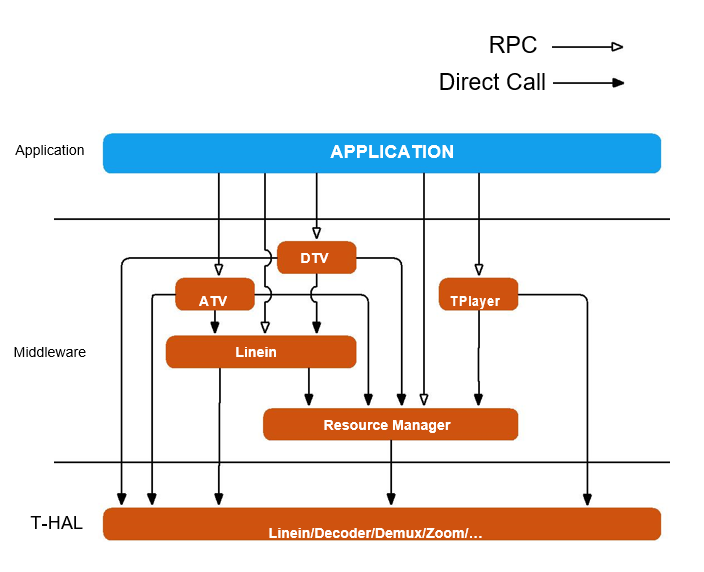
\includegraphics[width=10cm,height=11cm]{2.png}
\end{figure}
\centerline{{ 图 2.2: RM 模块上下文环境}}
 

\subsubsection{模块上下文环境}
\subsection{第1层设计}
   本章主要介绍 RM 的对外接口及主要使用场景的使用流程。
\subsubsection{接口设计}
    见接口文档。
\subsubsection{无冲突使用流程}
      图2.3描述了没有资源冲突的情况下,使用 RM 管理硬件资源的流程
\begin{figure}[h]
\centering
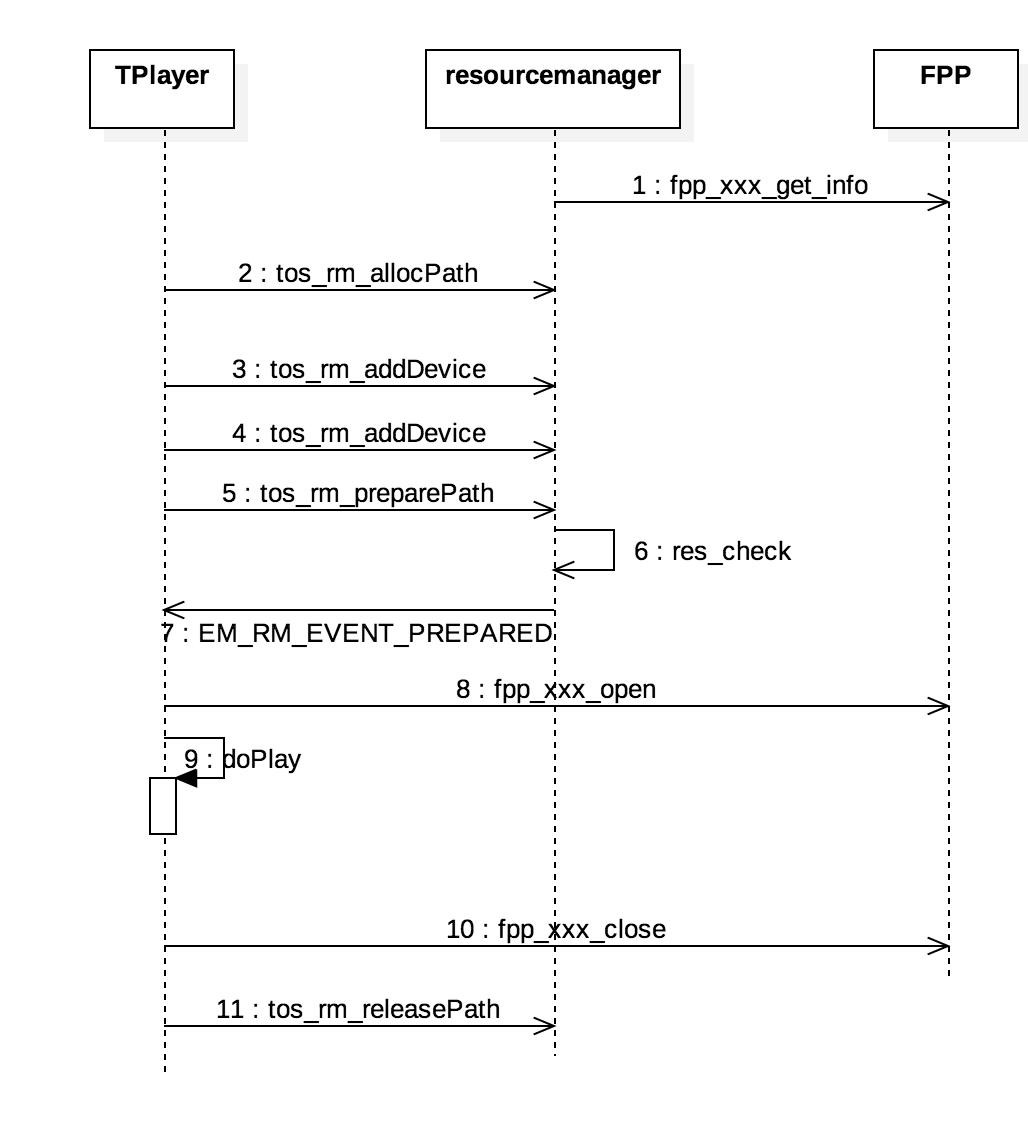
\includegraphics[width=10cm,height=10cm]{3.png}
\end{figure}

\centerline{{图 2.3: 无冲突使用流程}}
\begin{itemize}
\item 如步骤 3-4,TPlayer 从 RM 查询当前资源的使用情况,选择合适的资源(如满足需求的前提下,可用优先)添加到资源通道(Path)中。
\item 如步骤 6-8,RM 检查 Path 所有添加的资源,看是否有冲突,如果没有则发送 EM\_RM\_-EVENT\_PREPARED 消息给资源 TPlayer,告知资源申请成功。 
\item 如步骤 9-10,TPlayer 操作 FPP 接口控制资源进行播放等操作。
\item 如步骤 11-12,TPlayer 操作 FPP 接口释放资源控制,并告知 RM 释放硬件资源通道。
\item 后续的流程均在此流程基础上,增加额外的处理,部分正常流程可能在后续的图中省略。
\end{itemize}


\subsubsection{资源更新流程}
图2.4描述了资源正常使用过程中,因状态发生变化,需要更新资源的流程。如 DTV 换台,视频分辨率变化,视频出现了 HDR 信号,打开了 3D 等,都可能造成资源需求的变化。这时播放器可能需要更换更强大的设备(如果有)来满足播放,这种情况下我们通过先释放原来在用的设备,然后申请新设备来实现;也可能需要将另一个播放停下来才能满足需要,这种情况下我们通过额外的再占用一个设备,但不实际使用来实现。
\begin{figure}[h]
\centering
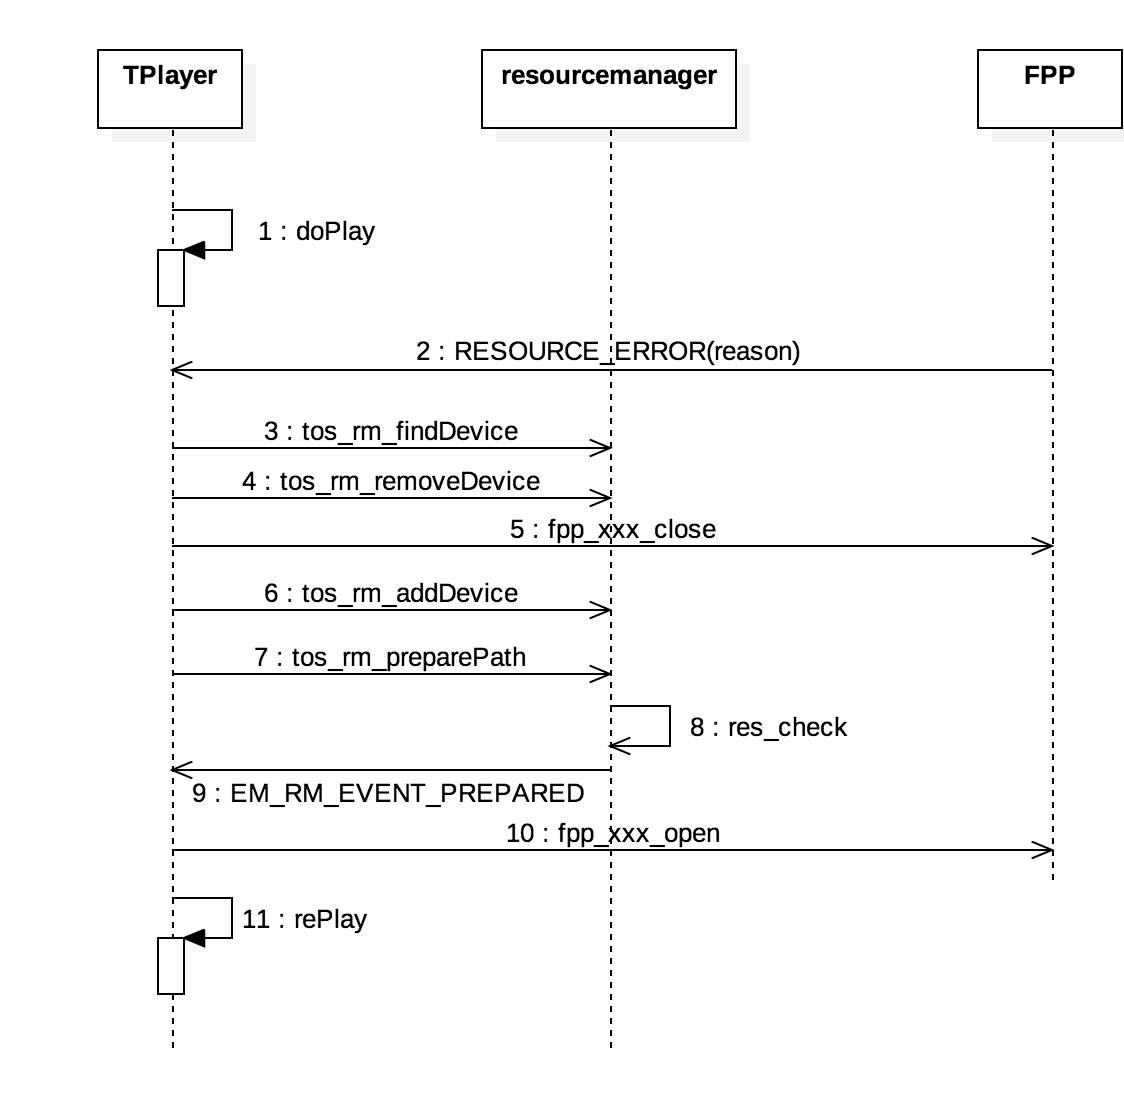
\includegraphics[width=10cm,height=10cm]{5.png}
\end{figure}

\centerline{{图 2.4: 资源更新流程}}

\begin{itemize}
\item 如步骤 1,TPlayer 已经完成了2.3的流程,开始播放了。
\item 如步骤 2,由于某些原因,FPP 发来消息告知由于设备冲突或者设备能力不足播放无法继续。 
\item 如步骤 3-6,TPlayer 从 RM 查询当前资源的使用情况,重新选择合适的资源,添加到到资源通道(Path)中。同时将不再需要的设备(如果有)关闭,并从资源通道移除。
\item 如步骤 7-9,RM 检查 Path 所有添加的资源,看是否有冲突,如果没有则发送 EM\_RM\_-EVENT\_PREPARED 消息给资源 TPlayer,告知资源申请成功。
\item 如步骤 10-11,TPlayer 操作新获取的设备,重新启动播放。
\end{itemize}


\subsubsection{资源冲突流程}
\begin{figure}[h]
\centering
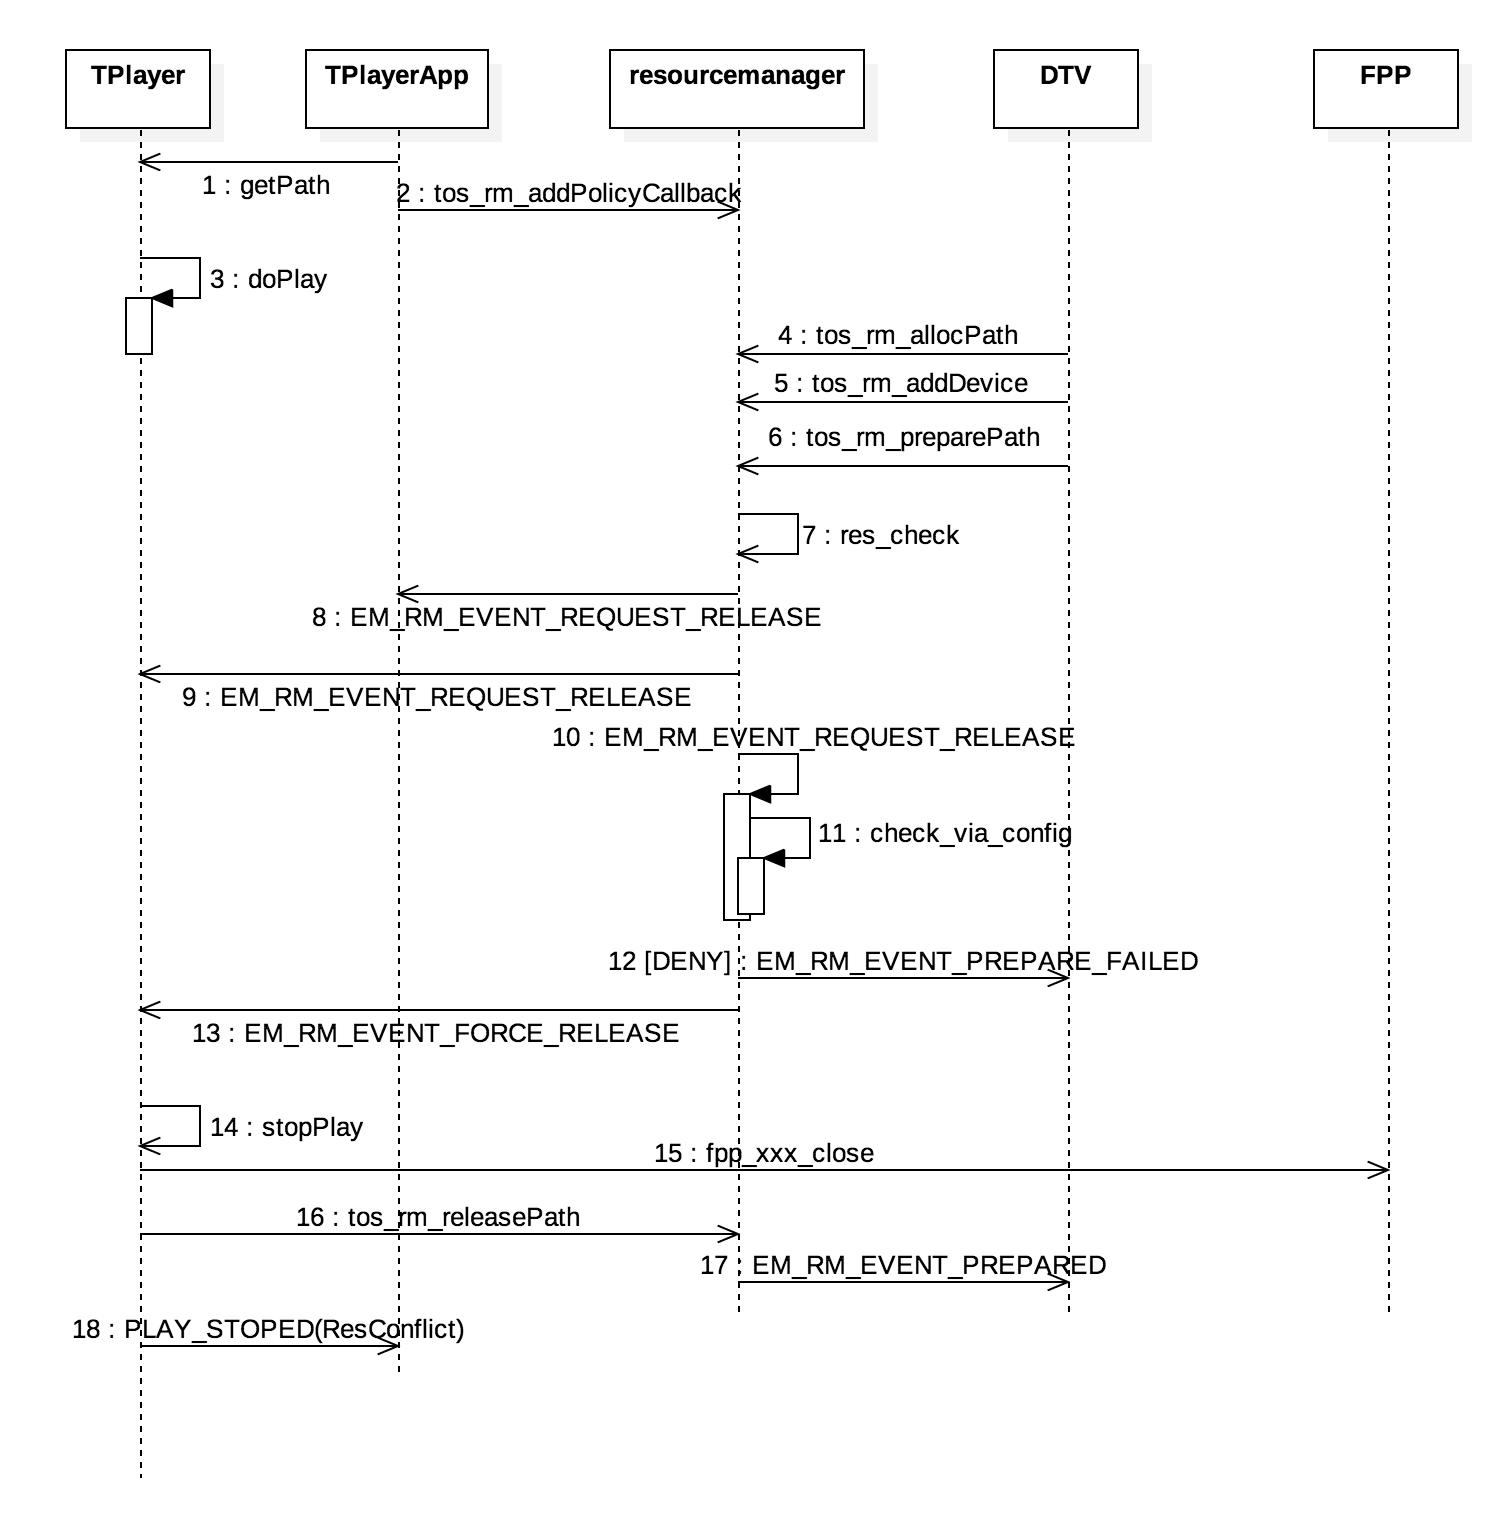
\includegraphics[width=10cm,height=10cm]{4.png}
\end{figure}

\centerline{{图 2.5: 资源冲突流程}}

\begin{itemize}
\item 如步骤 1-2,播放前,应用如果不满意默认的后来优先策略,可以获取 TPlayer 的 Path,然后注册 PolicyCallback, 定制资源重提策略。
\item 如步骤3,TPlayer已经完成了图2.3的流程,开始播放了。\
\item 如步骤4-7,DTV同时也按照图2.3的流程要开始播放。\
\item 如步骤8-12,RM发现DTV申请的资源跟TPlayer的有冲突,依次向TPlayer的应用,TPlayer及自己发出EM\_RM\_EVENT\_REQUEST\_RELEASE消息,请求释放资源。如果任何一个回返回了EM\_RM\_RESULT\_DENY,则RM会拒绝DTV的申请,向其发送EM\_RM\_RESULT\_PREPARE\_FAILED消息,DTV 播放失败;如果任何一个回调返回了EM\_RM\_RESULT\_CONFIRM,则 RM 会同意 DTV 的资源申请,向 TPlayer 发送 EM\_RM\_EVENT\_FORCE\_RELEASE 消息强制要求 TPlayer 释放资源;如果回调返回了 EM\_-RM\_RESULT\_TBD 则表示当前回调不做决定,依次交给下一个回调函数做决定。默认情况下,TPlayer 等资源使用者建议返回 EM\_RM\_RESULT\_TBD 不做决定,而 RM 会根据配置文件决定是否同意释放其它情况。 \
\item 如步骤 13-15,TPlayer 收到 EM\_RM\_EVENT\_FORCE\_RELEASE 消息后,必须马上停止播放,释放资源,并告知 RM。它可以通过 tos\_rm\_removeDevice 及 tos\_rm\_preparePath 仅释放指定资源,暂时保留其它资源以备稍后重新播放;也可以简单的通过 tos\_rm\_releasePath 释放所有资源。建议后者。\
\item 如步骤 16,资源释放成功后,RM 向 DTV 发送 EM\_RM\_EVENT\_PREPARED 消息,DTV即可按照图2.3的流程进行后续播放操作。\
\item 如步骤 17,TPlayer 告知 TPlayer 应用播放因为资源冲突而停止了。\
\end{itemize}


\subsubsection{重新播放流程}
图2.6描述了当资源恢复空闲有,如何恢复之前的播放(如果需要)的流程。
\begin{figure}[H]
\centering
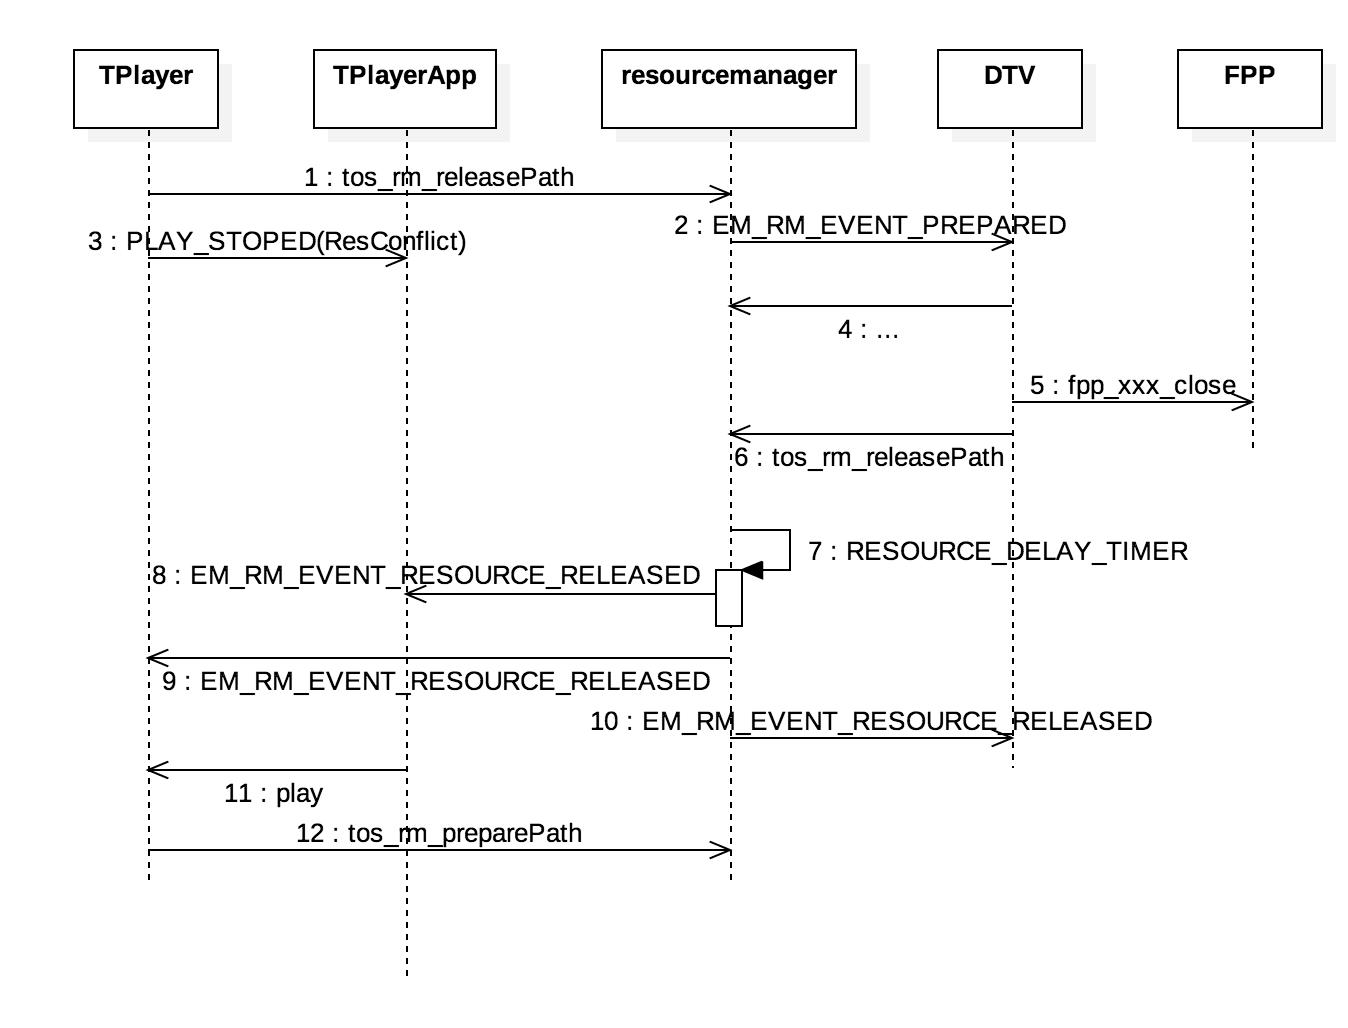
\includegraphics[height=3.5in]{6.png}

\end{figure}
\centerline{{图 2.6: 重新播放流程}}
\begin{itemize}
\item 如步骤1-4,接图2.5的流程,TPlayer播放因资源冲突播放停止,DTV开始播放。\
\item 如步骤5-6,DTV因为某些原因停止播放,释放了所有资源。(注:请尽量不要释放后马上有申请资源,如建议不要再换台释放,建议在切离DTV信源时释放)\
\item 如步骤7-10,RM在短暂延时后,发现如果没有新的使用者来申请这些设备,则向所有回调发送EM\_RM\_EVENT\_RESOURCE\_RELEASED消息,告知摩羯资源现状恢复空间了。一般来说,不建议使用者处理这个消息恢复播放,建议次消息应有应用来处理。 \
\item 如步骤11-12,TPlayer应用收到此消息后,重新调用TPlayer进行播放,TPlayer重走图2.3的流程。\
\end{itemize}
\end{document}